\documentclass{yann}
\yann{layout=onecolumn}
\yann{displaystyle}
\usepackage[most]{tcolorbox}
\usepackage{hyperref}



\newcommand{\Rpinf}{\Rp ∪\Acco{+∞}}
\newcommand{\sumni}{∑_{n=0}^{+∞}}
\newcommand{\Sanzn}{∑_n a_n z^n}
\newcommand{\Sanxn}{∑_n a_n x^n}
\newcommand{\Sbnzn}{∑_n b_n z^n}
\newcommand{\Scnzn}{∑_n c_n z^n}
\newcommand{\Ensembletq}[2]{\bigl\{#1\text{ tq }#2\bigr\}}
\newcommand{\me}{e} % {\mathrm{e}}
\newcommand{\I}{i} % {\mathrm{i}}

\begin{document}
\title{Séries entières}
\maketitle

% Rappeler du cours sur les séries de fonction \sum f_n convergence simple pour le domaine de définition et uniforme (convergence normale) pour les propriétés de continuité etc , 


Une série entière est une série de fonctions de la forme
$$\sum a_{n}z^{n}$$
où les coefficients $a_n$ forment une suite réelle ou complexe et $z$ une variable complexe.\\
Les séries entières possèdent des propriétés de convergence remarquables, qui s'expriment pour la plupart à l'aide de son rayon de convergence $R$, grandeur associée à la série. Sur le disque de convergence (disque ouvert de centre 0 et de rayon R), la fonction somme de la série peut être dérivée indéfiniment terme à terme.\\
Les séries entières sont 
\begin{enumerate}
\item un outil :
\begin{enumerate}
\item dans la résolution d'équations différentielles, par exemple $(1 + x)y' = αy$, en cherchant les solutions sous la forme $y(x)=\sum a_{n}x^{n}$,    
\item dans l'étude du comportement asymptotique d'un somme de variable aléatoires et la caractérisation d'une variable aléatoire par la fonction génératrice : $G_X(t)=\mathbb{E}[t^X]=\sum_{k=0}\mathbb {P} (X=k)t^{k}$,
\item dans la modélisation des systèmes dynamiques de manière discrète à l'aide de la transformée en $Z$, soit $s(n)$ l'état du système au temps $n$, sa transformée en $Z$ est
$$ S(z) = \mathcal{Z}\{s(n)\} =\sum_{n=-\infty}^{+\infty}s(n)z^{-n}.$$
\end{enumerate}
\item un objet préalable à l'analyse complexe des fonctions holomorphes et analytiques.
\end{enumerate}

\tableofcontents

\section{Généralités}

\Para{Définition}

On appelle \emph{série entière} toute série de fonctions de la forme $∑_n f_n$
où $(a_n)_{n∈ℂ}$ est une suite numérique et
où $\Fn{f_n}{ℂ}{ℂ}$ est définie par $f_n(z) = a_n z^n$.
La \emph{somme} de la série entière est la fonction \[ f \colon z \mapsto \sumni a_n z^n. \]
\Para{Exemple} La formule de la fonction exponentielle
$$e^{x}=\sum _{n=0}^{\infty }{\frac {x^{n}}{n!}}=1+x+{\frac {x^{2}}{2!}}+{\frac {x^{3}}{3!}}+\cdots .$$
\begin{figure}[!h]
\begin{center}
\includegraphics[width=2.5cm]{Exp_series-0.png}\includegraphics[width=2.5cm]{Exp_series-1.png}\includegraphics[width=2.5cm]{Exp_series-2.png}\includegraphics[width=2.5cm]{Exp_series-3.png}\includegraphics[width=2.5cm]{Exp_series-4.png}\includegraphics[width=2.5cm]{Exp_series-5.png}
\caption{La fonction exponentielle, $x\mapsto e^x$ en bleue, et la somme des $n+1$ termes de la série $\sum \frac{x^n}{n!}$ en rouge. }
\end{center}
\end{figure}

%Domaine de définition et convergence uniforme pour la continuité, dérivabilité
 
\Para{Lemme d'Abel}

Soit $\Sanzn$ une série entière et $z_0∈ℂ$ telle que la suite numérique $(a_n z_0^n)_{n∈ℕ}$ soit bornée.
Alors:
\begin{enumerate}
\item
  La série $\Sanzn$ converge absolument pour tout $z∈ℂ$ tel que $\Abs{z} < \Abs{z_0}$.
\item
  Plus précisément, la série de fonctions $\Sanzn$ converge normalement sur $\Ensembletq{z∈ℂ}{\Abs{z}≤r}$ dès que $0 ≤ r < \Abs{z_0}$.
\end{enumerate}




\Para{Attention!} Il n'y a pas toujours convergence normale (ni uniforme) sur $\Ensembletq{z∈ℂ}{\Abs{z}<\Abs{z_0}}$.



\Para{Définition}

Soit $\Sanzn$ une série entière.
Le \emph{rayon de convergence} $R∈\Rpinf$
de la série entière $\Sanzn$ est défini par
$$
  R = \sup \, \Bigl\{ \, r≥0 \text{ tel que} 
  \text{la suite de terme général } \Abs{a_n} r^n \text{ est bornée} \, \Bigr\}.$$

\Para{Corollaire}

Soit $\Sanzn$ une série entière de rayon de convergence $R$ et $z_0 ∈ℂ$.
\begin{itemize}
\item
  Si $\Abs{z_0} < R$,
  la série numérique $∑_n a_n z_0^n$ converge absolument.
\item
  Si $\Abs{z_0} > R$,
  la série numérique $∑_n a_n z_0^n$ diverge grossièrement;
  plus précisément, la suite $(a_n z_0^n)_{n∈ℕ}$ n'est pas bornée.
\item
  Si $\Abs{z_0} = R$, la série peut ou non converger.
\end{itemize}
\begin{figure}[!h]
\begin{center}
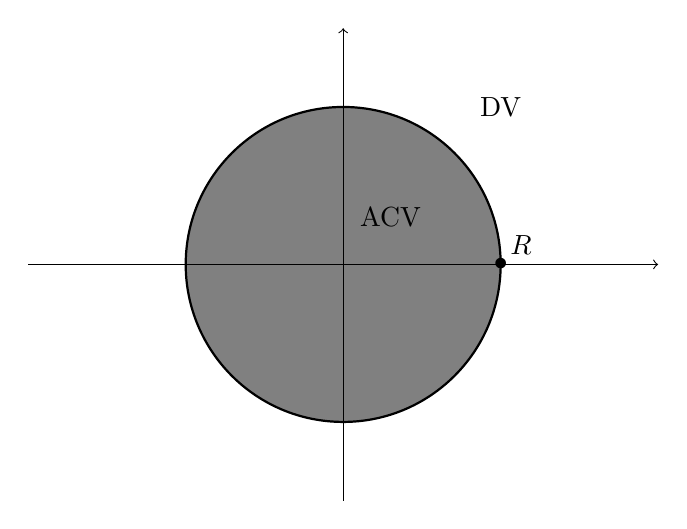
\begin{tikzpicture}[scale=2]
  \filldraw[thick,fill=gray] (0,0) circle (1) ;
  \draw[->] (-2,0) -- (2,0) ;
  \draw[->] (0,-1.5) -- (0,1.5) ;
  \draw (0.3,0.3) node {ACV};
  \draw (1,0) node {$\bullet$} node[above right] {$R$} ;
  \draw (1,1) node {DV};
\end{tikzpicture}
\caption{Disque de convergence d'une série entière}
\end{center}
\end{figure}


\Para{Définitions}

Soit $\Sanzn$ une série entière de rayon de convergence $R$.
\begin{itemize}
\item
  On appelle \emph{disque ouvert de convergence} de la série entière $\Sanzn$ l'ensemble
  \[ \Ensembletq{z∈ℂ}{\Abs{z}<R}. \]
\item
  On appelle \emph{cercle d'incertitude}
  (et parfois aussi, malheureusement, cercle de convergence)
  de la série entière $\Sanzn$ l'ensemble
  \[ \Ensembletq{z∈ℂ}{\Abs{z}=R}. \]
\end{itemize}



% -----------------------------------------------------------------------------
\section{Détermination du rayon de convergence}

\subsection{Avec le lemme d'Abel}

\Para{Proposition}

Soit $\Sanzn$ une série entière de rayon de convergence $R$.
Soit $z_0∈ℂ$.
\begin{itemize}
\item
  Si $(a_n z_0^n)$ est bornée, alors $R≥\Abs{z_0}$.
\item
  Si $∑_n \Abs{a_n z_0^n}$ diverge, alors $R≤\Abs{z_0}$.
\end{itemize}
\Para{Exemple} La rayon de convergence de la série entière $\sum x^n$ est 1 car
\begin{itemize}
\item la suite $(x^n)$ tend vers $0$ si $|x|<1$ (donc est bornée), donc $R≥1$,
\item la suite $(x^n)$ diverge si $|x|>1$, donc $R≤1$,
\end{itemize}
En conclusion  $R=1$.
\subsection{Avec d'Alembert}
Soit $\Sanzn$ une série entière et $R$ son rayon de convergence.
On suppose que:
\begin{itemize}
\item
  il existe $N∈ℕ$ tel que pour tout $n≥N$ on ait $a_n≠0$,
\item
  $\left|\frac{a_{n+1}}{a_n}\right| \Toninfℓ∈\Rpinf$.
\end{itemize}
Alors $R=1/ℓ$ si $l\neq 0$ et  $+\infty$ si $l=0$.
\Para{Exemple} La rayon de convergence de la série entière $\sum \frac{x^n}{n!}$ est $+\infty$ car
\begin{itemize}
\item la suite $(x^n)$ tend vers $0$ si $|x|<1$ (donc est bornée), donc $R≥1$,
\item la suite $(x^n)$ diverge si $|x|>1$, donc $R≤1$,
\end{itemize}
En conclusion  $R=1$.



\subsection{Avec les règles de comparaison}

\Para{Théorème}

Soit $\Sanzn$ et $\Sbnzn$ deux séries entières de rayons de convergence
respectivement $R_a$ et $R_b$.
\begin{enumerate}
\item
  S'il existe $α∈ℝ$ tel que $\Abs{a_n} = \GrandO \left( n^α\Abs{b_n} \right)$ quand $n\to+∞$, alors $R_a≥R_b$.
\item
  S'il existe $α∈ℝ$ et $K>0$ tel que $\Abs{a_n} \sim K n^α\Abs{b_n}$ quand $n\to+∞$, alors $R_a = R_b$.
\end{enumerate}

\pagebreak

% -----------------------------------------------------------------------------
\section{Opérations sur les séries entières}

\Para{Notations}
\begin{itemize}
\item
  Étant donné une série entière $\Sanzn$, on note $R_a$ son rayon de convergence et $f_a$ sa somme.
\item
  De même pour $\Sbnzn$ et $\Scnzn$.
\end{itemize}

\subsection{Somme}

\Para{Définition}

Soit $\Sanzn$ et $\Sbnzn$ deux séries entières.
On définit la \emph{somme} de ces deux séries entières
comme étant la série entière $\Scnzn$ où
\[ ∀n∈ℕ, \quad  c_n = a_n+b_n. \]

\Para{Proposition}

Dans ces conditions,
\begin{itemize}
\item
  $R_c≥\min(R_a,R_b)$ avec égalité si $R_a≠R_b$,
\item
  pour tout $z∈ℂ$ tel que $\Abs{z} < \min(R_a,R_b)$, on a $f_c(z) = f_a(z) + f_b(z)$.
\end{itemize}

\subsection{Multiplication par un scalaire}

\Para{Définition}

Soit $λ$ un scalaire et $\Sanzn$ une série entière.
On définit le \emph{produit} du scalaire et de la série entière
comme étant la série entière $\Sbnzn$ où
\[ ∀n∈ℕ, \quad  b_n =λa_n. \]

\Para{Proposition}

Dans ces conditions,
\begin{itemize}
\item
  $R_b = R_a$ si $λ≠0$, et $R_b = +∞$ si $λ= 0$,
\item
  pour tout $z∈ℂ$ tel que $\Abs{z} < R_a$, on a $f_b(z) =λf_a(z)$.
\end{itemize}

\subsection{Produit de Cauchy}

\Para{Définition}

Soit $\Sanzn$ et $\Sbnzn$ deux séries entières.
On définit le \emph{produit de Cauchy} de ces deux séries entières
comme étant la série entière $\Scnzn=\Sanzn\times\Sbnzn$ où
\[ ∀n∈ℕ, \quad c_n = ∑_{k=0}^n a_k b_{n-k}. \]

\Para{Proposition}

Dans ces conditions,
\begin{itemize}
\item
  $R_c ≥\min(R_a,R_b)$,
\item
  pour tout $z∈ℂ$ tel que $\Abs{z} < \min(R_a,R_b)$, on a $f_c(z) = f_a(z) f_b(z)$.
\end{itemize}

% -----------------------------------------------------------------------------
\section{Propriétés de la somme}

\Para{Théorème}[continuité sur le disque ouvert de convergence]

Soit $\Sanzn$ une série entière de rayon de convergence $R$ et de somme $f$.
Alors $f$ est continue sur le disque ouvert de convergence
\[ \Ensembletq{z∈ℂ}{\Abs{z}<R}. \]

\Para{Proposition}

Soit $\Sanzn$ une série entière de rayon de convergence $R$.
Alors les deux séries entières suivantes:
\begin{itemize}
\item
  la \og{}dérivée formelle\fg{} $∑_n b_n z^n$ où $b_n = (n+1)a_{n+1}$,
\item
  la \og{}primitive formelle\fg{} $∑_n c_n z^n$ où $c_n = \frac{a_{n-1}}{n}$
\end{itemize}
ont également un rayon de convergence égal à $R$.

\Para{Théorème}[primitivation terme à terme]

Soit $\Sanxn$ une série entière de rayon de convergence $R$ et de somme $f$.
Une primitive de $f$ sur $\intO{-R,R}$ est donnée par
\[ F \colon x \mapsto \sumni a_n \frac{x^{n+1}}{n+1} = ∑_{n=1}^{+∞} \frac{a_{n-1}}{n} x^n. \]

\Para{Proposition}[dérivation terme à terme]

Soit $\Sanxn$ une série entière de rayon de convergence $R$ et de somme $f$.
Alors $f$ est une fonction de classe $\CC1$ sur $\intO{-R,R}$
et $∀x∈\intO{-R,R}$,
\[ f'(x) = ∑_{n=1}^{+∞} n a_n x^{n-1} = \sumni (n+1) a_{n+1} \, x^n. \]

\Para{Théorème}[généralisation]

Soit $\Sanxn$ une série entière de rayon de convergence $R$ et de somme $f$.
Alors $f$ est une fonction de classe $\CC∞$ sur $\intO{-R,R}$
et $∀p∈ℕ$, $∀x∈\intO{-R,R}$,
\[ \begin{aligned} f^{(p)}(x)
    &= ∑_{n=p}^{+∞} a_n n(n-1) \cdots (n-p+1) x^{n-p} \\
    &= \sumni a_{n+p} \frac{(n+p)!}{n!} x^n.
\end{aligned} \]

\Para{Corollaire}

Soit $\Sanxn$ une série entière de rayon de convergence $R>0$ et de somme $f$.
Alors pour tout $n∈ℕ$, on a
\[ a_n = \frac{f^{(n)}(0)}{n!}. \]

% -----------------------------------------------------------------------------
\section{Fonctions développables en séries entières}

\Para{Notation}
\begin{itemize}
\item
  $I$ désigne un intervalle de $ℝ$ tel qu'il existe
  $ε> 0$ tel que $\intO{-ε,ε}⊂I$.
\end{itemize}

\Para{Définition}

Soit $\Fn fIℂ$.
On dit que $f$ est \emph{développable en série entière} au voisinage de $0$
si et seulement si il existe $α> 0$
et une série entière $\Sanxn$ de rayon de convergence $R≥α$ tels que
$\intO{-α,α}⊂I$ et
\[ ∀x∈\intO{-α,α} \+ f(x) = \sumni a_n x^n. \]

\Para{Proposition}

Si $\Fn fIℂ$ est développable en série entière au voisinage de $0$,
alors il existe $α> 0$ tel que
$f$ soit de classe $\CC∞$ sur $\intO{-α,α}$.

\Para{Définition}

Soit $\Fn fIℂ$ une fonction de classe $\CC∞$.
On appelle \emph{série de Taylor} de $f$ au voisinage de $0$
la série entière
\[ ∑_n a_n z^n \quad \text{où} \quad∀n∈ℕ\+ a_n = \frac{f^{(n)}(0)}{n!}. \]

\Para{Théorème}[unicité du développement en série entière]

Soit $\Fn fIℂ$ développable en série entière au voisinage de $0$.
Alors tout développement en série entière de $f$ au voisinage de $0$
est égal à sa série de Taylor au voisinage de $0$.

\Para{Corollaire}

Soit $\Fn fIℂ$ développable en série entière au voisinage de $0$.
Alors $f$ admet un développement limité au voisinage de $0$ à tout ordre,
et ce développement limité s'obtient en tronquant le développement en série entière.

\Para{Proposition}

Soit $\Fn fIℂ$.
Alors $f$ est développable en série entière au voisinage de $0$
si et seulement si il existe $α> 0$ tel que
\begin{itemize}
\item
  $f$ est de classe $\CC∞$ sur $\intO{-α,α}$,
\item
  la série de Taylor de $f$ converge sur $\intO{-α,α}$,
\item
  $f$ soit égale à la somme de se série de Taylor sur $\intO{-α,α}$.
\end{itemize}

% -----------------------------------------------------------------------------
\section{Fonctions usuelles}

\subsection{Exponentielle complexe}

\Para{Proposition}

La série entière $∑_n \frac{z^n}{n!}$ a un rayon de convergence infini.
Notons $φ\colon z \mapsto \sumni \frac{z^n}{n!}$ sa somme.
On montre successivement:
\begin{enumerate}
\item
  $∀(z_1,z_2)∈ℂ^2$, $φ(z_1+z_2) =φ(z_1)φ(z_2)$
\item
  $∀x∈ℝ$, $φ(x) = \me^x$
\item
  $∀θ∈ℝ$, $φ(\Iθ) = \cosθ+ \I \sinθ$
\item
  $∀(x,y)∈ℝ^2$, $φ(x+\I y) = \me^x(\cos y + \I \sin y)$
\end{enumerate}

\Para{Définition}

On appelle \emph{exponentielle} la fonction définie par
\[ ∀z∈ℂ, \quad \exp(z) = \sumni \frac{z^n}{n!}. \]
Il s'agit d'une série entière de rayon de convergence infini.
On note fréquemment $\me^z$ au lieu de $\exp(z)$.

\Para{Proposition}

Soit $z∈ℂ$ fixé et $\Fonction{φ}{ℝ}{ℂ}{t}{\exp(tz)}$\\
Alors $φ$ est de classe $\CC∞$ et
\[ ∀n∈ℕ \+ ∀t∈ℝ, \quad φ^{(n)}(t) = z^n \exp(tz). \]

\subsection{Trigonométrie}

\Para{Définitions}

On définit, pour tout $z∈ℂ$:
\begin{multicols}{2}
  \begin{itemize}
  \item
    $\cos z = \frac{\me^{\I z} + \me^{-\I z}}{2}$
  \item
    $\sin z = \frac{\me^{\I z} - \me^{-\I z}}{2\I}$
  \item
    $\ch z = \frac{\me^{z} + \me^{-z}}{2}$
  \item
    $\sh z = \frac{\me^{z} - \me^{-z}}{2}$
  \end{itemize}
\end{multicols}
Il s'agit de prolongement des fonctions cosinus, sinus, cosinus hyperbolique
et sinus hyperbolique, classiquement définies sur $ℝ$.

\Para{Proposition}

\begin{itemize}
\item
  Les formules usuelles de trigonométries restent valables,
  notamment $∀(a,b)∈ℂ^2$:
  \begin{itemize}
  \item
    $\cos(a+b) = \cos(a) \cos(b) - \sin(a) \sin(b)$
  \item
    $\sin(a+b) = \sin(a) \cos(b) + \cos(a) \sin(b)$
  \end{itemize}
\item
  On peut passer de la trigonométrie directe
  à la trigonométrie hyperbolique sachant que $∀z∈ℂ$:
  \begin{multicols}{2}
    \begin{itemize}
    \item
      $\ch(\I z) = \cos(z)$
    \item
      $\sh(\I z) = \I\sin(z)$
    \item
      $\cos(\I z) = \ch(z)$
    \item
      $\sin(\I z) = \I\sh(z)$
    \end{itemize}
  \end{multicols}
\end{itemize}

\Para{Proposition}

On a, pour tout $z∈ℂ$:
\begin{itemize}
\item
  $\DS \cos z  = ∑_{n=0}^{+∞} \frac{(-1)^n}{(2n)!} \, z^{2n}$
\item
  $\DS \sin z  = ∑_{n=0}^{+∞} \frac{(-1)^n}{(2n+1)!} \, z^{2n+1}$
\item
  $\DS \ch z = ∑_{n=0}^{+∞} \frac{1}{(2n)!} \, z^{2n}$
\item
  $\DS \sh z = ∑_{n=0}^{+∞} \frac{1}{(2n+1)!} \, z^{2n+1}$
\end{itemize}

Il s'agit de séries entières de rayon de convergence infini.

\subsection{$x \mapsto (1+x)^α$}

\Para{Proposition}

Soit $α∈ℝ$ et $\Fn{f}{\intO{-1,+∞}}{ℝ}$ définie par $f(x)=(1+x)^α$.
Alors $f$ est développable en série entière au voisinage de $0$.
Plus précisément, on a
\[ ∀x∈\intO{-1,1}, \quad (1+x)^α= ∑_{n=0}^{+∞} a_n x^n \]
où $a_0 = 1$ et \[ ∀n∈\Ns \+ a_n = \frac{1}{n!}∏_{k=0}^{n-1} (α-k). \]
On note parfois $a_n = \binom{α}{n}$.
Il s'agit d'une série entière de rayon de convergence égal à~1
si $α∉ℕ$, et $+∞$ si $α∈ℕ$.

\Para{Remarque}

Si $α∈ℤ$, le développement est également valable dans $ℂ$
\[ ∀z∈ℂ\text{ tel que } \Abs{z}<1, \quad
(1+z)^α=∑_{n=0}^{+∞} a_n z^n, \]
où $(a_n)_{n∈ℕ}$ est défini comme ci-dessus.

\Para{Exemple}

Déterminer le développement en série entière de la fonction $x\mapsto\arcsin x$.

\subsection{Fractions rationnelles}

\Para{Méthode}

Pour obtenir un développement en série entière (au voisinage de $0$)
d'une fraction rationnelle, on peut:
\begin{itemize}
\item
  la décomposer en éléments simples $\frac{1}{(x-a)^n}$ où $a∈ℂ^*$;
\item
  remarquer que $\frac{1}{(x-a)^n} = (-a)^{-n} \left[ 1+\left(-\frac xa\right) \right]^{-n}$;
\item
  se ramener à $(1+u)^α$.
\end{itemize}

On obtient une série entière de rayon de convergence~$\Abs{a}$.


\end{document}

% ------------------------------------------------------------------------------
% ------------------------------------------------------------------------------
% ------------------------------------------------------------------------------

\Exercice
\begin{enumerate}
\item
  Montrer que les deux intégrales
  $∫_0^1 \frac{\ln t}{1-t} \D t$ et
  $∫_0^1 \frac{\ln t}{1-t^2} \D t$ convergent.
\item
  En développant en série entière $\frac{1}{1-t}$ et $\frac{1}{1-t^2}$, calculer leurs valeurs.
\item
  En déduire $∫_0^{+∞} \frac{t\D t}{\sh t}$.
\end{enumerate}
